%----------------------------------------------------------------------------
\chapter{Hardverek}\label{sect:hardver}
%----------------------------------------------------------------------------

%Szöveg.

%,,,,,,,,,,,,,,,,,,,,,,,,,,,,,,,,,,,,,,,,,,,,,,,,,,,,,,,,,,,,,,,,,,,,,,,,,,,,
\section{Optikai megfontolások}\label{sect:hw_optikai}
%,,,,,,,,,,,,,,,,,,,,,,,,,,,,,,,,,,,,,,,,,,,,,,,,,,,,,,,,,,,,,,,,,,,,,,,,,,,,

Az optikai megfontolások közül az első a tekintetkövetés során felhasznált fénytartomány, ami lehet a látható fény tartománya, valamint az infratartomány. A második fontos szempont pedig a kamera látószöge, ami alapjaiban határozza meg a felhasználótól megkívánt beavatkozás mértékét, valamint a szem felbontását (ezzel közvetve az elérhető maximális pontosságot).

\bigskip

A \textbf{látható fényben} történő követés egyértelmű előnye, hogy nem igényel speciális hardvert, a legtöbb, a piacon kapható analóg vagy digitális (web)kamera ebben a tartományban ,,lát''. Sőt, a digitális eszközökben a CMOS/CCD érzékelő elé szinte minden esetben ún. infratükröt (felülvágó szűrőt, amely kirekeszti a látható fény feletti spektrumot) helyeznek, ezeket az eszközöket tehát sikerrel csak látható fényben használhatjuk. A látható fény használatakor azonban nem feledkezhetünk meg annak hátrányairól sem: a követéshez analizálandó kép meglehetősen érzékeny lesz a megfelelő megvilágításra. A fényviszonyok változásának kiküszöbölése komolyabb előfeldolgozást kíván, és extrém esetekben nem is mindig teljesíthető.

\begin{figure}[!ht]
\centering
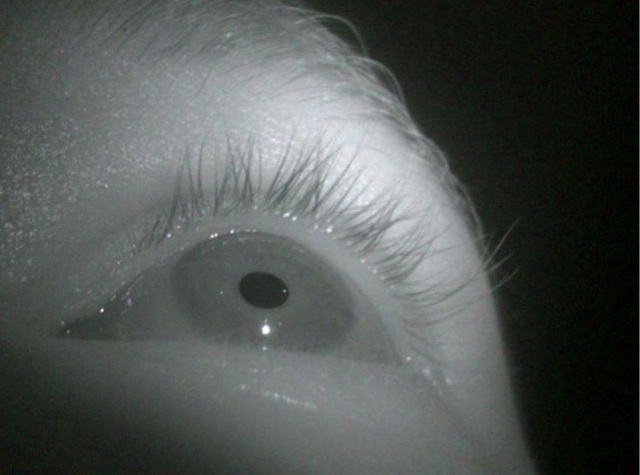
\includegraphics[width=100mm, keepaspectratio]{figures/infra_eye.png}
\caption{Az emberi szem képe infravörös fényben. Forrás: \url{http://bit.ly/aKwzsZ}}
\label{fig:eyepic}
\end{figure}

Az \textbf{infratartománynak} a látható fénnyel szemben vannak előnyei, és hátrányai is. Az előnyök közé tartozik, hogy a pupilla képe a infra megvilágításban nagyon kontrasztos (lásd \figref{eyepic} ábra), jóval könnyebben szegmentálható az írisztől (különösen sötétebb szemű alany esetén), mint látható fényben. Az infrás megvalósítás hátránya azonban, hogy a megfelelő működéshez sötétet igényel (igaz, ezzel összhangban a látható megvilágítási változásokra invariáns), de sötétben, a tisztán infra megvilágítás megvalósítása nehéz feladat, különösen a piacon kapható egyszerűbb infra LED-ekkel, vagy LED-es reflektorokkal.

\bigskip

A követéshez használt kamera optikája lehet egyrészt \textbf{nagylátószögű}. Ez azzal az előnnyel jár, hogy a vizsgálat alatt álló személy fejmozgása szabadabb lehet, nincs szükség a fejpozíció fixálására (pl. álltámasszal). A szemrégió külön szegmentálható, majd ezen régión belül a pupillát követve valósulhat meg a tekintetkövetés. A módszer hátránya, hogy a szemrégió nem tölti be az egész képet, vagyis nem használja ki maximálisan a rendelkezésre álló felbontást. Ennek következtében a tekintetkövetés pontossága jelentős mértékben romolhat, esetleg lehetetlenné is válhat.

További lehetőség a \textbf{teleobjektívek}, vagyis zoomoptikák használata. Teleobjektívvel a szemrégió ,,közel hozható'' még nagy távolságról is, hogy teljesen kitöltse a feldolgozandó képet, kihasználva annak teljes felbontását. Ez azonban azzal a hátránnyal jár, hogy a fejet fix pozícióba kell kényszeríteni (pl. egy álltámasz segítségével), ugyanis a fej mozgásával a pupillarégió kikerülhet a kamera látószögéből.

Végül lehetőség nyílik egyfajta ,,hibrid'' megoldás használatára is, amelynél 

%............................................................................
%\subsection{Analóg TV-kamera}\label{sect:analog}
%............................................................................

%,,,,,,,,,,,,,,,,,,,,,,,,,,,,,,,,,,,,,,,,,,,,,,,,,,,,,,,,,,,,,,,,,,,,,,,,,,,,
%\section{Összefoglalás}\label{sect:hardver_osszefoglalas}
%,,,,,,,,,,,,,,,,,,,,,,,,,,,,,,,,,,,,,,,,,,,,,,,,,,,,,,,,,,,,,,,,,,,,,,,,,,,,

%Összefoglalás.